%
%
% Author:
% Efraín Soto Apolinar.
% http://www.aprendematematicas.org/
% 
% This document contains the definition of
% two commands to include Yellow notes in 
% the margin of a page.
%


\documentclass[12pt]{article}
\usepackage{color}
\usepackage{tikz}
\usepackage{calc}
\usepackage{mnote}

\setlength{\parskip}{0ex}
\setlength{\parindent}{0ex}
\usepackage{flowchart}
\usepackage{tikz}
\pagestyle{empty}
\usetikzlibrary{calc,shapes,arrows,shapes.multipart}

\newlength{\yellownotewidth}
\setlength{\yellownotewidth}{2.5cm}
\newlength{\yellownoteheight}
\setlength{\yellownoteheight}{2.5cm}
%   -   -   -   -   -   -   -   -   -   -   -   -
% Yellow note...
%   -   -   -   -   -   -   -   -   -   -   -   -
\newcommand{\yellownote}[1]{
	\marginpar{
		\vspace{-0.5\yellownoteheight}
		\begin{center}
			\begin{tikzpicture}
				\draw[white,fill=gray!25,opacity=0.75,shift={(-0.125,-0.125)}] 
				(0,0) rectangle (\yellownotewidth,\yellownoteheight);
				\draw[fill=yellow!35] (0,0) rectangle (\yellownotewidth,\yellownoteheight);
				\draw[opacity=0.45,fill=gray!50] (0.7\yellownotewidth,0) -- 
				(0.9\yellownotewidth,0.45) -- (\yellownotewidth,0.4) -- cycle;
				\node[blue,below] at (0.5\yellownotewidth,\yellownoteheight) {
					\begin{minipage}{\yellownotewidth-1em}
						\scriptsize\sf#1
					\end{minipage}
				};
			\end{tikzpicture}
		\end{center}
		\vspace{0.5\yellownoteheight}
	}
}

%   -   -   -   -   -   -   -   -   -   -   -   -
% Resizeable - Yellow note...
%   -   -   -   -   -   -   -   -   -   -   -   -
\newcommand{\resizeableyellownote}[3]{
	\setlength{\yellownotewidth}{#1cm}
	\setlength{\yellownoteheight}{#2cm}
	\marginpar{
		\vspace{-0.5\yellownoteheight}
		\begin{center}
			\begin{tikzpicture}
				\draw[white,fill=gray!25,opacity=0.75,shift={(-0.125,-0.125)}] 
				(0,0) rectangle (\yellownotewidth,\yellownoteheight);
				\draw[fill=yellow!35] (0,0) rectangle (\yellownotewidth,\yellownoteheight);
				\draw[opacity=0.45,fill=gray!50] (0.7\yellownotewidth,0) -- 
				(0.9\yellownotewidth,0.45) -- (\yellownotewidth,0.4) -- cycle;
				\node[blue,below] at (0.5\yellownotewidth,\yellownoteheight) {
					\begin{minipage}{\yellownotewidth-1em}
						\scriptsize\sf#3
					\end{minipage}
				};
			\end{tikzpicture}
		\end{center}
		\vspace{0.5\yellownoteheight}
	}
}
%
% Fonts
%
\usepackage{slantsc}
\usepackage[sc]{mathpazo}
%
%
%
\begin{document}
	%
	%
	%
	To include a yellow note into a document insert the 
	code:
	\begin{verbatim}
		\yellownote{
			Message into a yellow note. We just want to see how it 
			will look.
		}
	\end{verbatim}
	and you will see the first yellow note at the 
	margin of the page.
	\yellownote{
		Message into a yellow note. We just want to see how it 
		will look.
	}
	Include more text then...
	
	
	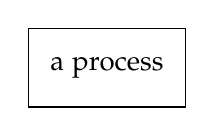
\begin{tikzpicture}
		\node (JohnDeer) [draw, process, minimum width=2cm, minimum height=1cm] {a process 	};
	
	\end{tikzpicture}


	
	This text is only a test. This text is only a test. 
	This text is only a test. This text is only a test. 
	This text is only a test. This text is only a test. 
	This text is only a test. This text is only a test. 
	This text is only a test. This text is only a test. 
	This text is only a test. This text is only a test. 
	This text is only a test. This text is only a test. 
	This text is only a test. This text is only a test. 
	
	And when neccesary, change the size of the yellow note 
	with the following command:
	\begin{verbatim}
		\resizeableyellownote{2.5}{1.5}{
			Resizeable yellow note.
		}
	\end{verbatim}
	to get the second one... 
	\resizeableyellownote{2.5}{1.5}{Resizeable yellow note.}
	Each of the arguments are: \verb|{width}{height}| 
	in centimeters. You do not need to include the 
	unit in the argument. The instruction already 
	knows it. 
	This text is only a test. This text is only a test. 
	This text is only a test. This text is only a test. 
	This text is only a test. This text is only a test. 
	This text is only a test. This text is only a test. 
	This text is only a test. This text is only a test. 
	This text is only a test. This text is only a test. 
	This text is only a test. This text is only a test. 
	This text is only a test. This text is only a test. 
	
	I hope this help you improve your design.
	
\end{document}
